%%%%%%%%%%%%%%%%%%%%%%%%%%%
\newcommand{\documentName} { Hoja 3.09 }
\newcommand{\documentContent} { Funciones } 
\newcommand{\waterMark} { } 
%%%%%%%%%%%%%%%%%%%%%%%%%%%

% Configuración del documento.
\newcommand{\schoolSubject} { Matemáticas 3º ESO - Recuperación}
\newcommand{\school} { IES La Serna }
\newcommand{\academicPeriod} { Curso 2020/2021 }


\newcommand{\autor} { Andrés Giménez Muñoz }
\newcommand{\emailAuthor} { agimenezmunoz@ieslaserna.com }
\newcommand{\autorSing}{ Profesores: Andrés } 
\renewcommand{\schoolSubject} { Examen Matemáticas 2º ESO  }
\renewcommand{\school} { IES José de Churriguera  }
\renewcommand{\academicPeriod} { Curso 2022/2023 }

\renewcommand{\autor} { Andrés Giménez Muñoz }
\renewcommand{\emailAuthor} { andresprofemates@outlook.es }
\renewcommand{\autorSing}{ Profesor: Andrés } 

%%%%%%%%%%%%%%%%%%%%%%%%%%%
% Exam configuration
\pointsdroppedatright   %% No mostrar la puntuación
%\pointsinrightmargin % Para poner las puntuaciones a la derecha. Se puede cambiar. Si se comenta, sale a la izquierda.
%\extrawidth{-1.5cm} %Un poquito más de margen por si ponemos textos largos.
%\marginpointname{ \emph{\points}}

%% Si se comenta no aparecerán los espacios de la solución.
%\nocancelspace

%% Esto es de la clase exam. Si dejamos sin comentar \printanswers, se mostraran las soluciones. 
%% Si la comentamos y dejamos sin comentar \noprintanswers, pues no se muestran las soluciones.
%\printanswers
%\noprintanswers

%%%%%%%%%%%%%%%%%%%%%%%%%%%

\usepackage{eqparbox}
\usepackage{pgfplots}
\usepackage{pgfplotstable}
\pgfplotsset{compat=1.16}

\usepackage{pgfplots}
\pgfplotsset{compat=1.6}

\pgfplotsset{soldot/.style={color=red,only marks,mark=*}} \pgfplotsset{holdot/.style={color=red,fill=white,only marks,mark=*}}

\pgfplotsset{
    % Global Styles
    % axis lines = middle,
    % xlabel = $x$,
    % ylabel = $y$,
    % no markers,
    % samples=50,
    % grid = both,
    trig format plots=rad,
    grid style={dashed, gray!30},
    %enlargelimits = false,
    %axis line style = {line width=0.5pt},
    % every axis plot/.append style={
    %     line width = 1.25pt,
    %     smooth,
    %     },
    % Label every pi
    halves/.style={
    xtick = {-12.5664, -10.9956, -9.42478, -7.85398, -6.28319, -4.71239, -3.14159, -1.5708, 0, 1.5708, 3.14159, 4.71239, 6.28319, 7.85398, 9.42478, 10.9956, 12.5664, 14.1372, 15.708, 17.2788, 18.8496, 20.4204, 21.9911, 23.5619, 25.1327},
    xticklabels = {$-4\pi$,$-\frac{7\pi}{2}$,$-3\pi$,$-\frac{5\pi}{2}$,$-2\pi$,$-\frac{3\pi}{2}$,$-\pi$,$-\frac{\pi}{2}$,$0$,$\frac{\pi}{2}$,$\pi$,$\frac{3\pi}{2}$,$2\pi$,$\frac{5\pi}{2}$,$3\pi$,$\frac{7\pi}{2}$,$4\pi$,$\frac{9\pi}{2}$,$5\pi$,$\frac{11\pi}{2}$,$6\pi$,$\frac{13\pi}{2}$,$7\pi$,$\frac{15\pi}{2}$,$8\pi$}
    },
    % Label every pi
    wholes/.style={
    xtick = {-12.5664, -9.42478, -6.28319, -3.14159, 0., 3.14159, 6.28319, 9.42478, 12.5664, 15.708, 18.8496, 21.9911, 25.1327},
    xticklabels = {$-4\pi$,$-3\pi$,$-2\pi$,$-\pi$,$0$,$\pi$,$2\pi$,$3\pi$,$4\pi$,$5\pi$,$6\pi$,$7\pi$,$8\pi$}
    },
    soldot/.style={color=red,only marks,mark=*},
    holdot/.style={color=red,fill=white,only marks,mark=*}
}


\begin{document}
\begin{questions}
    \question
    Data la función $f(x)=x^2+2x-3$.
    \begin{parts}
        \part
        Calcula $f(3)$, $f(-1)$, $f(0)$ y $f(-4)$.
        \part
        ¿Existe algún valor de $x$ para el que $f(x)=-2$? ¿Y para el que $f(x)=-6$?
    \end{parts}

    \question
    Haz una tabla de valores y representa la función.
    \begin{equation*}
        f(x)= \left\{ \begin{array}{lcc}
            x+1 & si & x \leq 1 \\
            \\ -2x+3 &  si & 1 < x \\
        \end{array}
        \right.
    \end{equation*}
    \begin{parts}
        \part
        Indica si es continua, de no ser así ¿Cuáles son los puntos de discontinuidad y cuánto vale la función en dichos puntos?
        \part
        Indica los intervalos de crecimiento y decrecimiento.
        \part
        Indica cuales son los máximos y los mínimos y si son relativos y absolutos.
    \end{parts}

    % \question
    % Haz una tabla de valores y representa la función.
    % \begin{equation*}
    %     f(x)= \left\{ \begin{array}{lcc}
    %         5 & si & x \leq 2 \\
    %         \\ x^2-6x+10 &  si & 2 < x < 5 \\
    %         \\ 4x-15 &  si  & x \geq 5
    %     \end{array}
    %     \right.
    % \end{equation*}
    % \begin{parts}
    %     \part
    %     Indica si es continua, de no ser así ¿Cuales son los puntos de discontinuidad y cuánto vale la función en dichos puntos?
    %     \part
    %     Indica los intervalos de crecimiento y decrecimiento.
    %     \part
    %     Indica cuales son los máximos y los mínimos y si son relativos y absolutos.
    % \end{parts}

    \question
    El entrenador de un corredor está tomando tiempos y en los primeros $12 s$ obtiene la siguiente tabla:
    \begin{table}[h!]
        \centering
        \begin{tabular}{|c|c|c|c|c|c|c|c|}
            \hline
            \cellcolor[gray]{0.8}Tiempo en (s)         & 0 & 3  & 4  & 6  & 10 & 12 \\
            \hline
            \cellcolor[gray]{0.8}Espacio recorrido (m) & 0 & 21 & 28 & 42 & 70 & 84 \\
            \hline
        \end{tabular}
    \end{table}
    \begin{parts}
        \part
        Representa la función en una tabla.
        \part
        ¿Cuántos metros ha recorrido en 5s?
        \part
        ¿Cuánto tarda en recorrer los primeros 50 m?
    \end{parts}

    % \question
    % % Hay que revisar este problema.
    % Una taxista llamado Juan, nos cobra $7,75\euro{}$ por la bajada de bandera más $3,33\euro{}$ por kilometro, 
    % mientras que Pedro, nos cobra $4,6\euro{}$ por la bajada de banderas más $3,5\euro{}$ el kilometro.
    % ¿Con cual nos interesa desplazarnos en función de los kilometros que queramos realizar? 

    \newpage
    \question
    Indica los intervalos de crecimiento y decrecimiento, máximos y mínimos y puntos de discontinuidad, si los tiene, de las siguientes funciones \textbf{lineales}. \\
    \small *Observar como el coeficiente del término en $x$ indica la pendiente de la recta.
    \normalsize

    \begin{multicols}{2}
        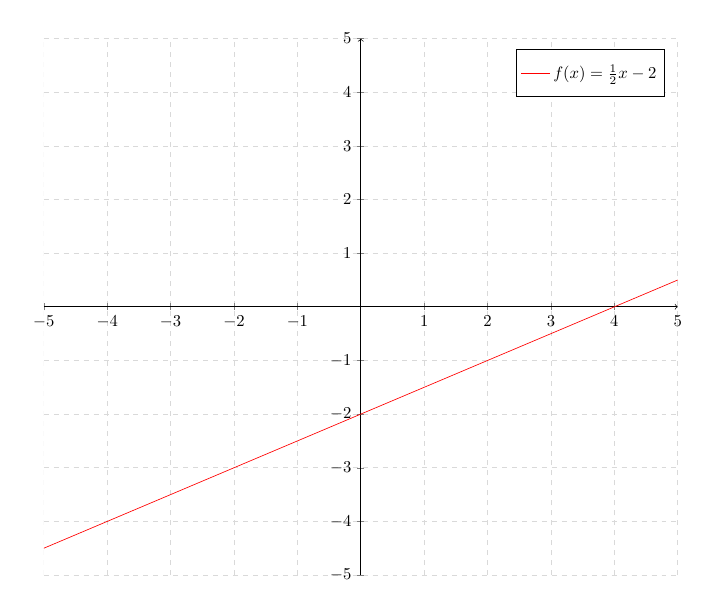
\begin{tikzpicture}[scale=0.6]
            \begin{axis}[
                    %title={$f(x)=x^2$},
                    axis lines=middle,
                    axis line style={->},
                    legend style={inner ysep=7pt},
                    %x label style={at={(axis description cs:0.5,-0.06)},anchor=north},
                    %y label style={at={(axis description cs:-0.06,.5)},rotate=90,anchor=south},
                    %xlabel={Nº de bombillas},ylabel={Vida en horas},
                    grid,
                    width=15cm,
                    xmax=5,ymax=5,xmin=-5,ymin=-5,
                    %axis lines=middle
                ]
                \addplot [mark=, samples = 50, red] {0.5*x-2};
                \addlegendentry{$f(x)=\frac{1}{2}x-2$}
            \end{axis}
        \end{tikzpicture}

        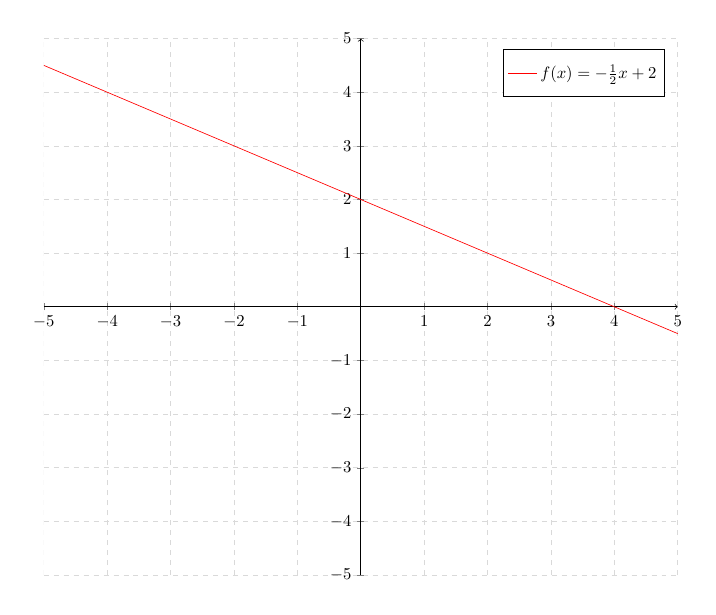
\begin{tikzpicture}[scale=0.6]
            \begin{axis}[
                    %title={$f(x)=x^2$},
                    axis lines=middle,
                    axis line style={->},
                    legend style={inner ysep=7pt},
                    %x label style={at={(axis description cs:0.5,-0.06)},anchor=north},
                    %y label style={at={(axis description cs:-0.06,.5)},rotate=90,anchor=south},
                    %xlabel={Nº de bombillas},ylabel={Vida en horas},
                    grid,
                    width=15cm,
                    xmax=5,ymax=5,xmin=-5,ymin=-5,
                    %axis lines=middle
                ]
                \addplot [mark=, samples = 50, red] {-0.5*x+2};
                \addlegendentry{$f(x)=-\frac{1}{2}x+2$}
            \end{axis}
        \end{tikzpicture}
    \end{multicols}

    \begin{multicols}{2}
        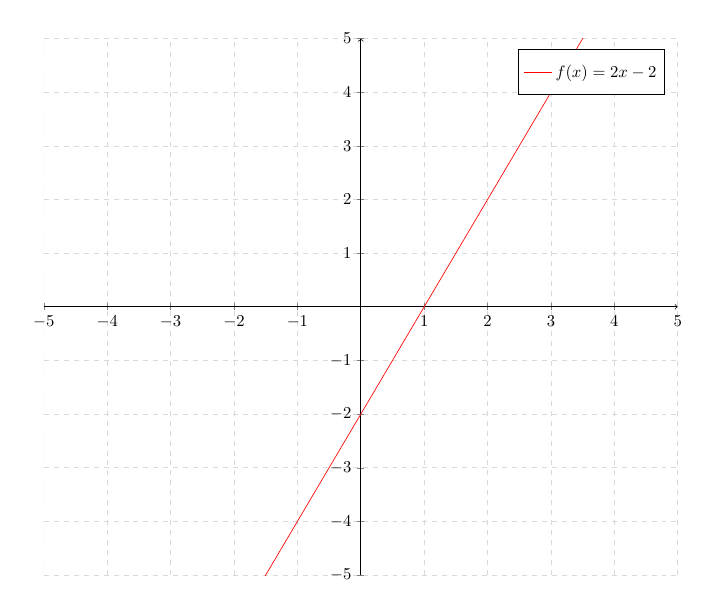
\begin{tikzpicture}[scale=0.6]
            \begin{axis}[
                    %title={$f(x)=x^2$},
                    axis lines=middle,
                    axis line style={->},
                    legend style={inner ysep=7pt},
                    %x label style={at={(axis description cs:0.5,-0.06)},anchor=north},
                    %y label style={at={(axis description cs:-0.06,.5)},rotate=90,anchor=south},
                    %xlabel={Nº de bombillas},ylabel={Vida en horas},
                    grid,
                    width=15cm,
                    xmax=5,ymax=5,xmin=-5,ymin=-5,
                    %axis lines=middle
                ]
                \addplot [mark=, samples = 50, red] {2*x-2};
                \addlegendentry{$f(x)=2x-2$}
            \end{axis}
        \end{tikzpicture}

        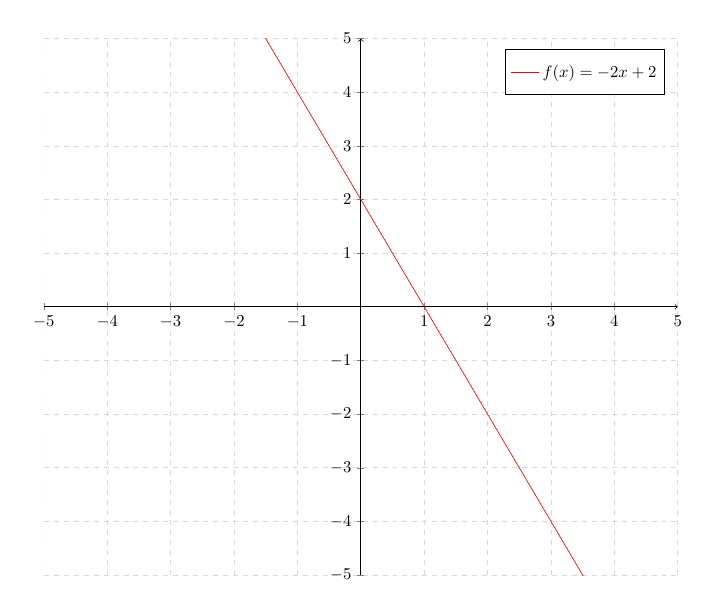
\begin{tikzpicture}[scale=0.6]
            \begin{axis}[
                    %title={$f(x)=x^2$},
                    axis lines=middle,
                    axis line style={->},
                    legend style={inner ysep=7pt},
                    %x label style={at={(axis description cs:0.5,-0.06)},anchor=north},
                    %y label style={at={(axis description cs:-0.06,.5)},rotate=90,anchor=south},
                    %xlabel={Nº de bombillas},ylabel={Vida en horas},
                    grid,
                    width=15cm,
                    xmax=5,ymax=5,xmin=-5,ymin=-5,
                    %axis lines=middle
                ]
                \addplot [mark=, samples = 50, red] {-2*x+2};
                \addlegendentry{$f(x)=-2x+2$}
            \end{axis}
        \end{tikzpicture}
    \end{multicols}

    \newpage
    \question
    Indica los intervalos de crecimiento y decrecimiento, máximos y mínimos y puntos de discontinuidad, si los tiene, de las siguientes funciones \textbf{polinómicas}.

    \begin{multicols}{2}
        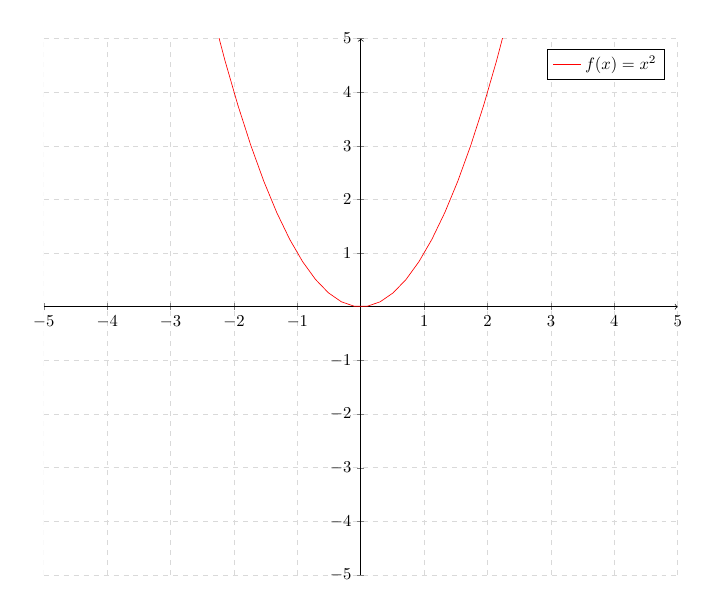
\begin{tikzpicture}[scale=0.6]
            \begin{axis}[
                    %title={$f(x)=x^2$},
                    axis lines=middle,
                    axis line style={->},
                    %x label style={at={(axis description cs:0.5,-0.06)},anchor=north},
                    %y label style={at={(axis description cs:-0.06,.5)},rotate=90,anchor=south},
                    %xlabel={Nº de bombillas},ylabel={Vida en horas},
                    grid,
                    width=15cm,
                    xmax=5,ymax=5,xmin=-5,ymin=-5,
                    %axis lines=middle
                ]
                \addplot [mark=, samples = 50, red] {x^2};
                \addlegendentry{$f(x)=x^2$}
            \end{axis}
        \end{tikzpicture}

        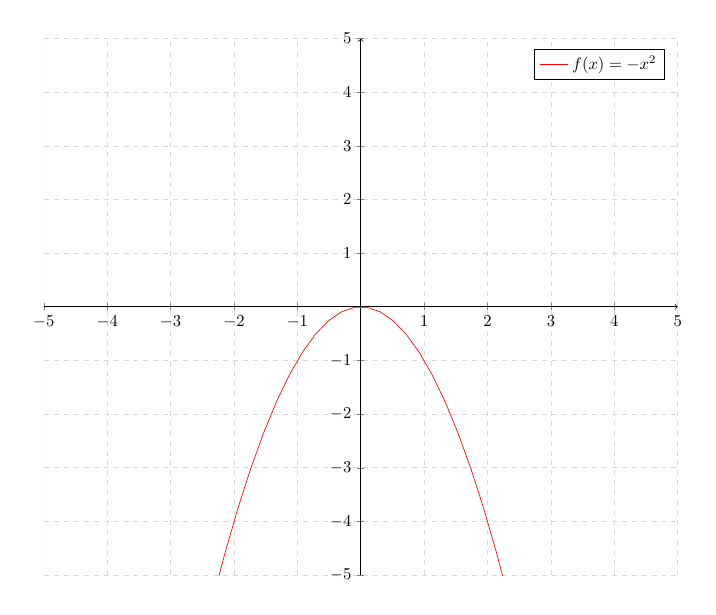
\begin{tikzpicture}[scale=0.6]
            \begin{axis}[
                    %title={$f(x)=-x^2$},
                    axis lines=middle,
                    axis line style={->},
                    %x label style={at={(axis description cs:0.5,-0.06)},anchor=north},
                    %y label style={at={(axis description cs:-0.06,.5)},rotate=90,anchor=south},
                    %xlabel={Nº de bombillas},ylabel={Vida en horas},
                    grid,
                    width=15cm,
                    xmax=5,ymax=5,xmin=-5,ymin=-5,
                    %axis lines=middle
                ]
                \addplot [mark=, samples = 50, red] {-x^2};
                \addlegendentry{$f(x)=-x^2$}
            \end{axis}
        \end{tikzpicture}
    \end{multicols}

    \begin{multicols}{2}
        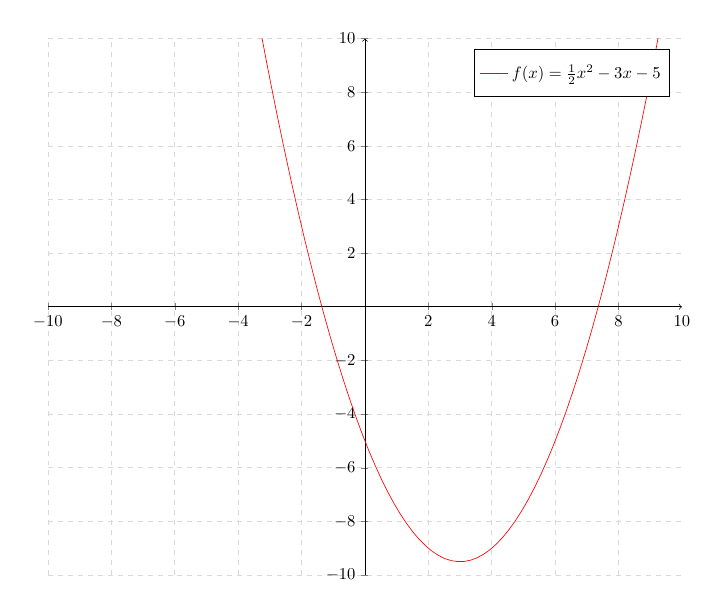
\begin{tikzpicture}[scale=0.6]
            \begin{axis}[
                    %title={$f(x)=x^2-10$},
                    axis lines=middle,
                    axis line style={->},
                    legend style={inner ysep=7pt},
                    %x label style={at={(axis description cs:0.5,-0.06)},anchor=north},
                    %y label style={at={(axis description cs:-0.06,.5)},rotate=90,anchor=south},
                    %xlabel={Nº de bombillas},ylabel={Vida en horas},
                    grid,
                    width=15cm,
                    xmax=10,ymax=10,xmin=-10,ymin=-10,
                    %axis lines=middle
                ]
                \addplot [mark=,  domain = -10:10, samples=100, red] {0.5*x^2-3*x-5};
                \addlegendentry{$f(x)=\frac{1}{2}x^2-3x-5$}
            \end{axis}
        \end{tikzpicture}

        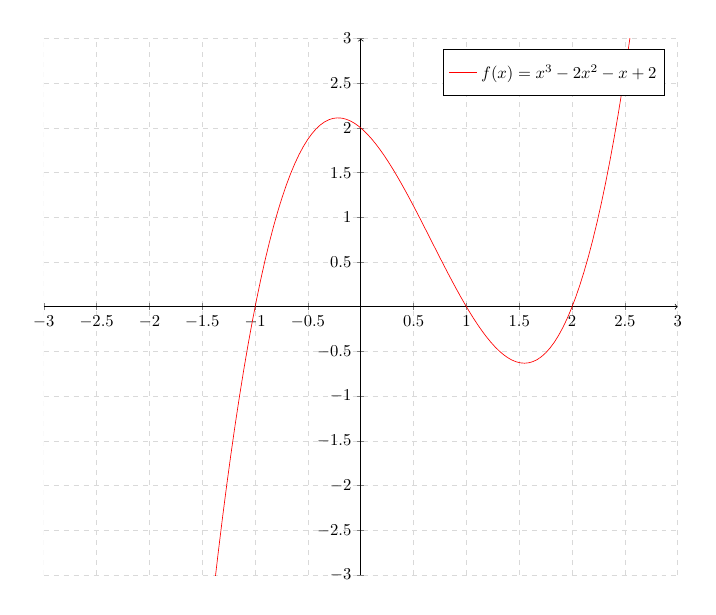
\begin{tikzpicture}[scale=0.6]
            \begin{axis}[
                    %title={$f(x)=x^2-10$},
                    axis lines=middle,
                    axis line style={->},
                    legend style={inner ysep=7pt},
                    %x label style={at={(axis description cs:0.5,-0.06)},anchor=north},
                    %y label style={at={(axis description cs:-0.06,.5)},rotate=90,anchor=south},
                    %xlabel={Nº de bombillas},ylabel={Vida en horas},
                    no markers,
                    grid,
                    width=15cm,
                    xmax=3,ymax=3,xmin=-3,ymin=-3,
                    %axis lines=middle
                    % restrict y to domain=-20:20
                ]
                \addplot [mark= thick,  domain = -3:3, samples=150, red] {x^3-2*x^2-x+2};
                \addlegendentry{$f(x)=x^3-2x^2-x+2$}
            \end{axis}
        \end{tikzpicture}
    \end{multicols}

    \begin{multicols}{2}
        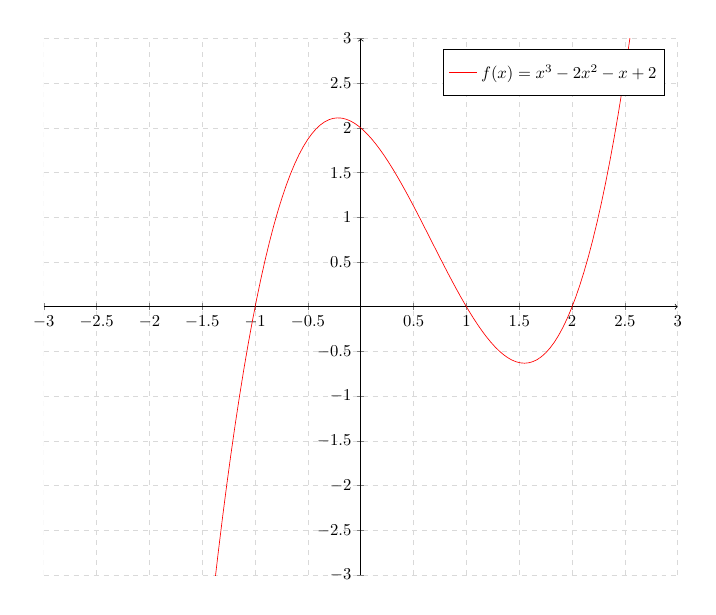
\begin{tikzpicture}[scale=0.6]
            \begin{axis}[
                    %title={$f(x)=x^2-10$},
                    axis lines=middle,
                    axis line style={->},
                    legend style={inner ysep=7pt},
                    %x label style={at={(axis description cs:0.5,-0.06)},anchor=north},
                    %y label style={at={(axis description cs:-0.06,.5)},rotate=90,anchor=south},
                    %xlabel={Nº de bombillas},ylabel={Vida en horas},
                    no markers,
                    grid,
                    width=15cm,
                    xmax=3,ymax=3,xmin=-3,ymin=-3,
                    %axis lines=middle
                    % restrict y to domain=-20:20
                ]
                \addplot [mark= thick,  domain = -3:3, samples=150, red] {x^3-2*x^2-x+2};
                \addlegendentry{$f(x)=x^3-2x^2-x+2$}
            \end{axis}
        \end{tikzpicture}

        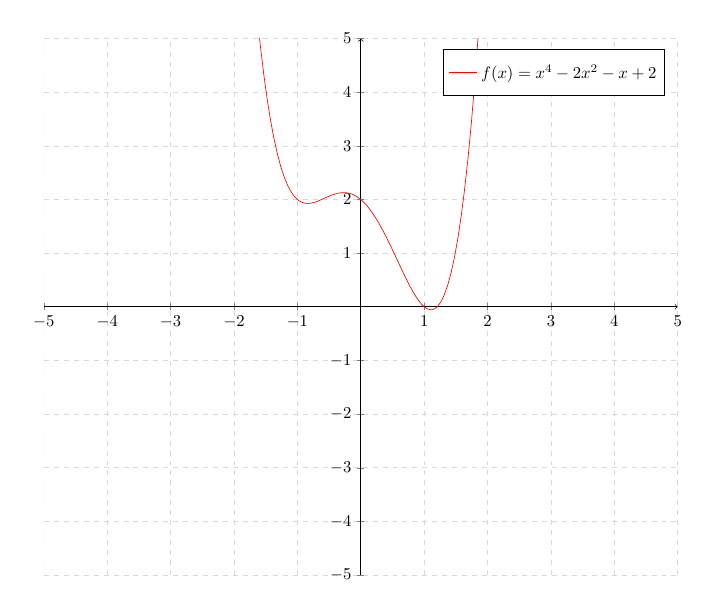
\begin{tikzpicture}[scale=0.6]
            \begin{axis}[
                    %title={$f(x)=x^2-10$},
                    axis lines=middle,
                    axis line style={->},
                    legend style={inner ysep=7pt},
                    %x label style={at={(axis description cs:0.5,-0.06)},anchor=north},
                    %y label style={at={(axis description cs:-0.06,.5)},rotate=90,anchor=south},
                    %xlabel={Nº de bombillas},ylabel={Vida en horas},
                    no markers,
                    grid,
                    width=15cm,
                    xmax=5,ymax=5,xmin=-5,ymin=-5,
                    %axis lines=middle
                    % restrict y to domain=-20:20
                ]
                \addplot [mark= thick,  domain = -4:4, samples=150, red] {x^4-2*x^2-x+2};
                \addlegendentry{$f(x)=x^4-2x^2-x+2$}
            \end{axis}
        \end{tikzpicture}
    \end{multicols}

    \newpage

    \newpage
    \question
    Indica los intervalos de crecimiento y decrecimiento, máximos y mínimos y puntos de discontinuidad, si los tiene, de las siguientes funciones.

    \begin{multicols}{2}
        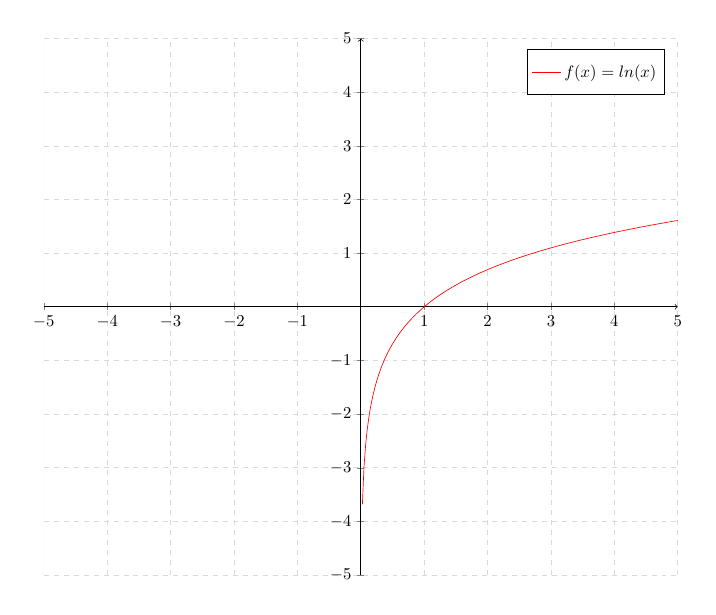
\begin{tikzpicture}[scale=0.6]
            \begin{axis}[
                    %title={$f(x)=x^2-10$},
                    axis lines=middle,
                    axis line style={->},
                    legend style={inner ysep=7pt},
                    %x label style={at={(axis description cs:0.5,-0.06)},anchor=north},
                    %y label style={at={(axis description cs:-0.06,.5)},rotate=90,anchor=south},
                    %xlabel={Nº de bombillas},ylabel={Vida en horas},
                    no markers,
                    grid,
                    width=15cm,
                    xmax=5,ymax=5,xmin=-5,ymin=-5,
                    %axis lines=middle
                    % restrict y to domain=-20:20
                ]
                \addplot [mark= thick,  domain = 0:5, samples=200, red] {ln(x)};
                \addlegendentry{$f(x)=ln(x)$}
            \end{axis}
        \end{tikzpicture}

        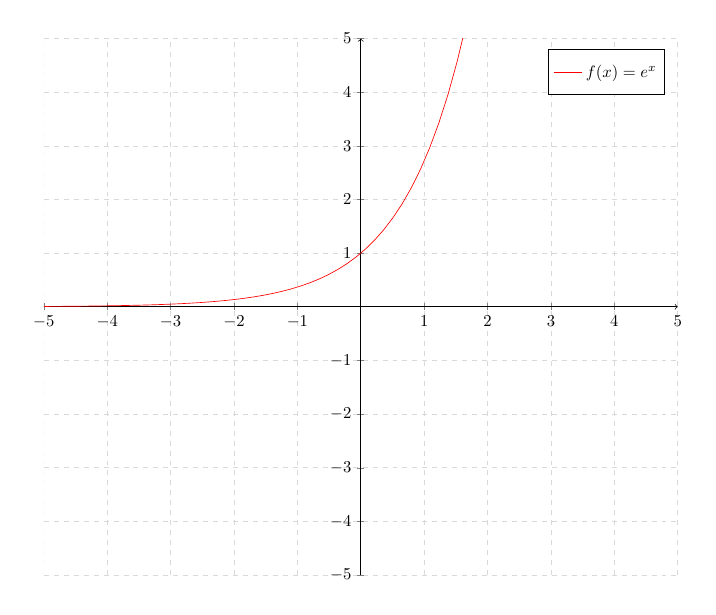
\begin{tikzpicture}[scale=0.6]
            \begin{axis}[
                    %title={$f(x)=x^2-10$},
                    axis lines=middle,
                    axis line style={->},
                    legend style={inner ysep=7pt},
                    %x label style={at={(axis description cs:0.5,-0.06)},anchor=north},
                    %y label style={at={(axis description cs:-0.06,.5)},rotate=90,anchor=south},
                    %xlabel={Nº de bombillas},ylabel={Vida en horas},
                    no markers,
                    grid,
                    width=15cm,
                    xmax=5,ymax=5,xmin=-5,ymin=-5,
                    %axis lines=middle
                    % restrict y to domain=-20:20
                ]
                % \addplot [mark= thick,  domain = -6:6, samples=20, red] {x^4-5*x^2+4};
                \addplot [mark= thick,  domain = -5:5, samples=70, red] {exp(x)};
                \addlegendentry{$f(x)=e^x$}
            \end{axis}
        \end{tikzpicture}
    \end{multicols}

    \begin{multicols}{2}
        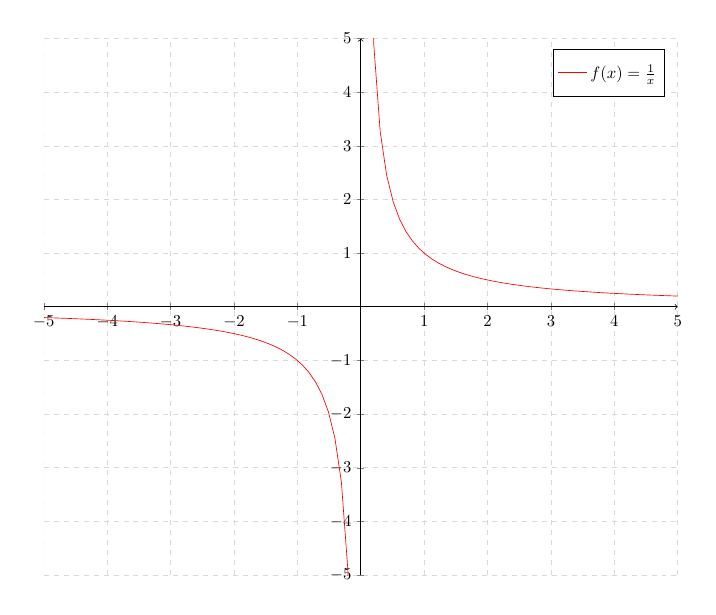
\begin{tikzpicture}[scale=0.6]
            \begin{axis}[
                    %title={$f(x)=x^2-10$},
                    axis lines=middle,
                    axis line style={->},
                    legend style={inner ysep=7pt},
                    %x label style={at={(axis description cs:0.5,-0.06)},anchor=north},
                    %y label style={at={(axis description cs:-0.06,.5)},rotate=90,anchor=south},
                    %xlabel={Nº de bombillas},ylabel={Vida en horas},
                    no markers,
                    grid,
                    width=15cm,
                    xmax=5,ymax=5,xmin=-5,ymin=-5,
                    %axis lines=middle
                    restrict y to domain=-20:20
                ]
                %\addplot [color=green, mark=] {x};
                \addplot [mark= thick,  domain = -5:0, samples=50, red] {1/x};
                \addplot [mark= thick,  domain = 0:5, samples=50, red] {1/x};
                \addlegendentry{$f(x)=\frac{1}{x}$}
            \end{axis}
        \end{tikzpicture}

        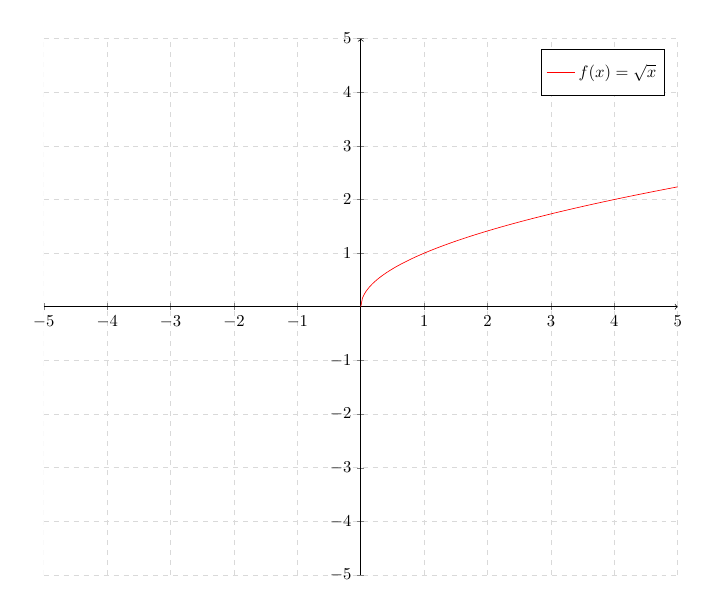
\begin{tikzpicture}[scale=0.6]
            \begin{axis}[
                    %title={$f(x)=x^2-10$},
                    axis lines=middle,
                    axis line style={->},
                    legend style={inner ysep=7pt},
                    %x label style={at={(axis description cs:0.5,-0.06)},anchor=north},
                    %y label style={at={(axis description cs:-0.06,.5)},rotate=90,anchor=south},
                    %xlabel={Nº de bombillas},ylabel={Vida en horas},
                    no markers,
                    grid,
                    width=15cm,
                    xmax=5,ymax=5,xmin=-5,ymin=-5,
                    %axis lines=middle
                    % restrict y to domain=-20:20
                ]
                \addplot [mark= thick,  domain = 0:5, samples=200, red] {sqrt(x)};
                \addlegendentry{$f(x)=\sqrt{x}$}
            \end{axis}
        \end{tikzpicture}
    \end{multicols}

    \newpage
    \question
    Indica los intervalos de crecimiento y decrecimiento, máximos y mínimos y puntos de discontinuidad, si los tiene, de las siguientes funciones \textbf{trigonométricas}.

    \begin{multicols}{2}
        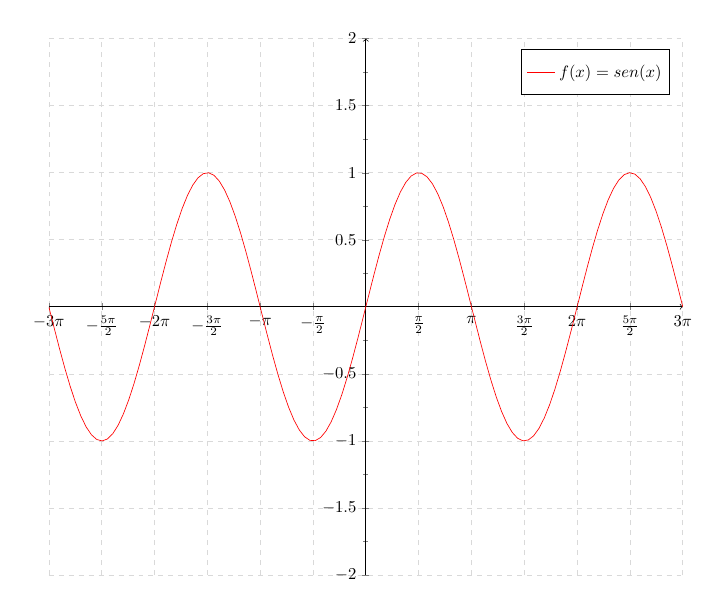
\begin{tikzpicture}[scale=0.6]
            \begin{axis}[
                    halves,
                    minor tick num = 1,
                    %title={$f(x)=x^2-10$},
                    axis lines=middle,
                    axis line style={->},
                    legend style={inner ysep=7pt},
                    %x label style={at={(axis description cs:0.5,-0.06)},anchor=north},
                    %y label style={at={(axis description cs:-0.06,.5)},rotate=90,anchor=south},
                    %xlabel={Nº de bombillas},ylabel={Vida en horas},
                    no markers,
                    grid,
                    width=15cm,
                    xmax=3*pi,ymax=2,xmin=-3*pi,ymin=-2,
                    %axis lines=middle
                    % restrict y to domain=-20:20
                ]
                \foreach \x/\xtext in {0, 3.14/\pi{}, 1, 1.5/\frac{3}{2}, 2};
                \addplot [mark= thick,  domain = -3*pi:3*pi, samples=120, red] {sin(x)};
                \addlegendentry{$f(x)=sen(x)$};

            \end{axis}
        \end{tikzpicture}

        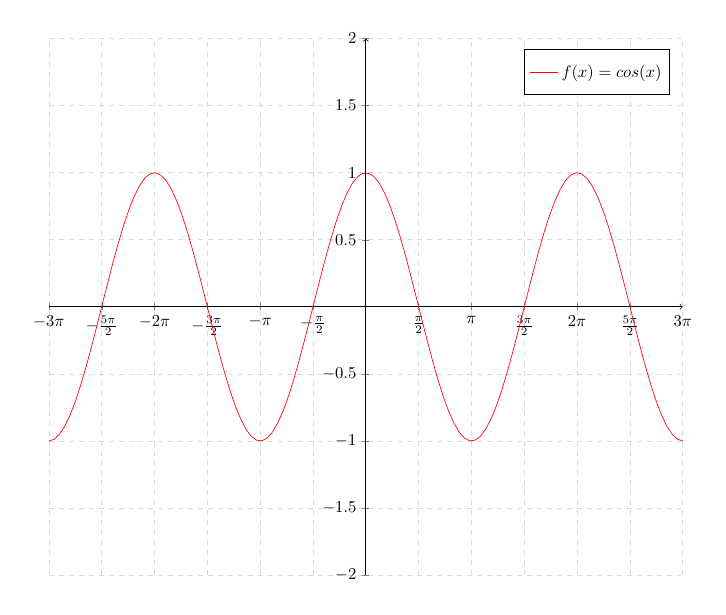
\begin{tikzpicture}[scale=0.6]
            \begin{axis}[
                    halves,
                    %title={$f(x)=x^2-10$},
                    axis lines=middle,
                    axis line style={->},
                    legend style={inner ysep=7pt},
                    %x label style={at={(axis description cs:0.5,-0.06)},anchor=north},
                    %y label style={at={(axis description cs:-0.06,.5)},rotate=90,anchor=south},
                    %xlabel={Nº de bombillas},ylabel={Vida en horas},
                    no markers,
                    grid,
                    width=15cm,
                    xmax=3*pi,ymax=2,xmin=-3*pi,ymin=-2,
                    %axis lines=middle
                    % restrict y to domain=-20:20
                ]
                \addplot [mark= thick,  domain = -3*pi:3*pi, samples=120, red] {cos(x)};
                \addlegendentry{$f(x)=cos(x)$}
            \end{axis}
        \end{tikzpicture}
    \end{multicols}

    \begin{multicols}{2}
        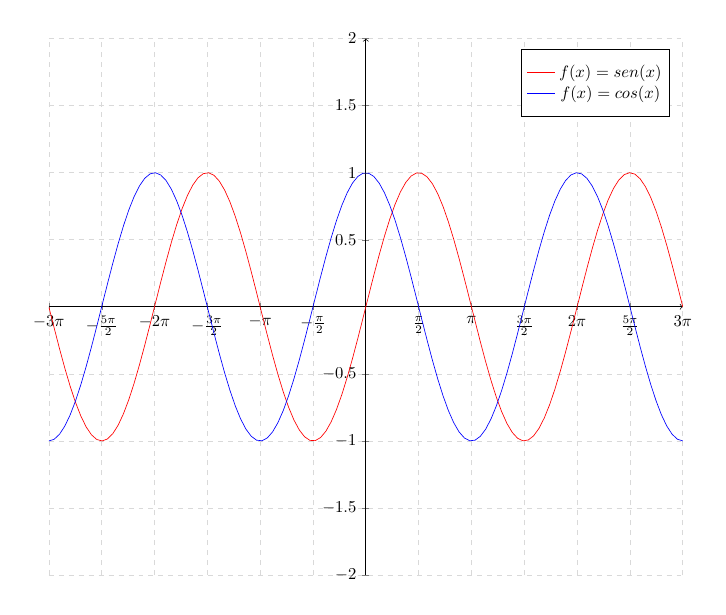
\begin{tikzpicture}[scale=0.6]
            \begin{axis}[
                    halves,
                    %title={$f(x)=x^2-10$},
                    axis lines=middle,
                    axis line style={->},
                    legend style={inner ysep=7pt},
                    %x label style={at={(axis description cs:0.5,-0.06)},anchor=north},
                    %y label style={at={(axis description cs:-0.06,.5)},rotate=90,anchor=south},
                    %xlabel={Nº de bombillas},ylabel={Vida en horas},
                    no markers,
                    grid,
                    width=15cm,
                    xmax=3*pi,ymax=2,xmin=-3*pi,ymin=-2,
                    %axis lines=middle
                    % restrict y to domain=-20:20
                ]
                \addplot [mark= thick,  domain = -3*pi:3*pi, samples=120, red] {sin(x)};
                \addplot [mark= thick,  domain = -3*pi:3*pi, samples=120, blue] {cos(x)};
                \addlegendentry{$f(x)=sen(x)$}
                \addlegendentry{$f(x)=cos(x)$}
            \end{axis}
        \end{tikzpicture}

        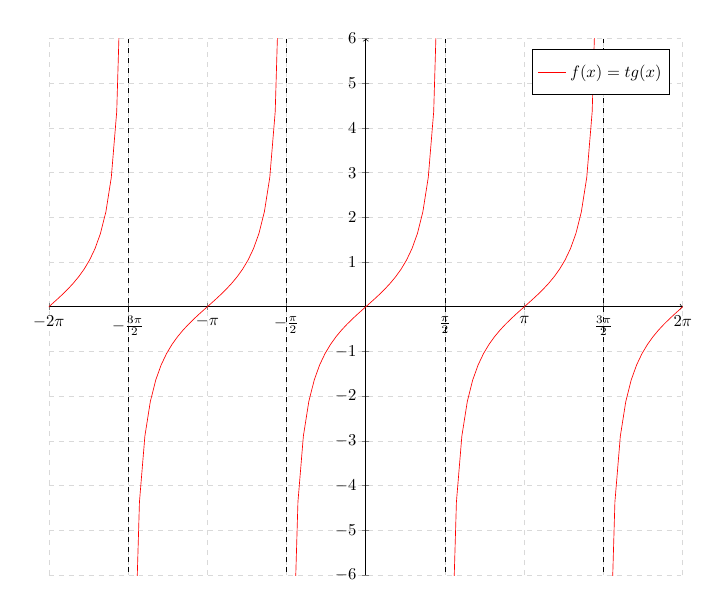
\begin{tikzpicture}[scale=0.6]
            \begin{axis}[
                    halves,
                    %title={$f(x)=x^2-10$},
                    axis lines=middle,
                    axis line style={->},
                    legend style={inner ysep=7pt},
                    %x label style={at={(axis description cs:0.5,-0.06)},anchor=north},
                    %y label style={at={(axis description cs:-0.06,.5)},rotate=90,anchor=south},
                    %xlabel={Nº de bombillas},ylabel={Vida en horas},
                    no markers,
                    grid,
                    width=15cm,
                    xmax=2*pi,ymax=6,xmin=-2*pi,ymin=-6,
                    %axis lines=middle
                    % restrict y to domain=-20:20
                ]
                \addplot [mark= thick,  domain = -5*pi/2+0.01:-3*pi/2-0.01, samples=30, red] {tan(x)};
                \addplot [mark= thick,  domain = -3*pi/2+0.01:-pi/2-0.01, samples=30, red] {tan(x)};
                \addplot [mark= thick,  domain = -pi/2+0.01:pi/2-0.01, samples=30, red] {tan(x)};
                \addplot [mark= thick,  domain = pi/2+0.01:3*pi/2-0.01, samples=30, red] {tan(x)};
                \addplot [mark= thick,  domain = 3*pi/2+0.01:5*pi/2-0.01, samples=30, red] {tan(x)};

                \draw[dashed] (axis cs:-3*pi/2,6) -- (axis cs:-3*pi/2,-6);
                \draw[dashed] (axis cs:-pi/2,6) -- (axis cs:-pi/2,-6);
                \draw[dashed] (axis cs:pi/2,6) -- (axis cs:pi/2,-6);
                \draw[dashed] (axis cs:3*pi/2,6) -- (axis cs:3*pi/2,-6);

                \addlegendentry{$f(x)=tg(x)$}
            \end{axis}
        \end{tikzpicture}

    \end{multicols}

    \newpage
    \question
    Indica los intervalos de crecimiento y decrecimiento, máximos y mínimos y puntos de discontinuidad, si los tiene, de las siguientes funciones.
    \begin{multicols}{2}
        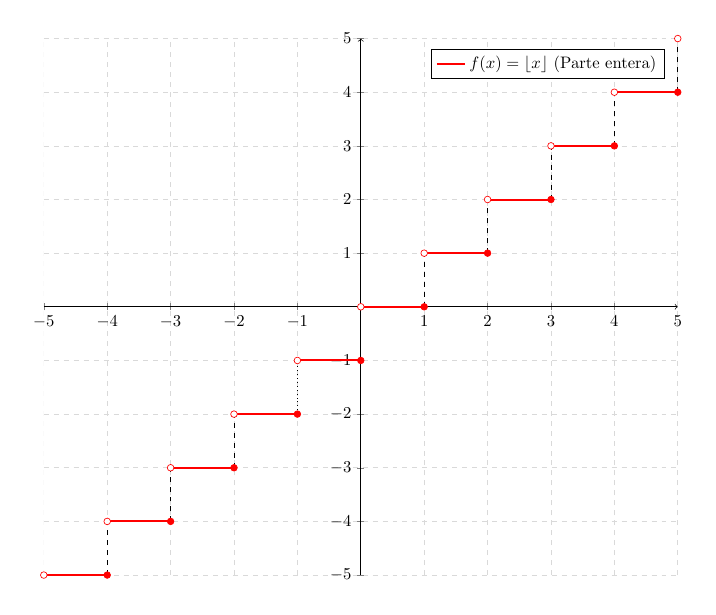
\begin{tikzpicture}[scale=0.6]
            \begin{axis}[
                    %title={$f(x)=-x^2$},
                    axis lines=middle,
                    axis line style={->},
                    %x label style={at={(axis description cs:0.5,-0.06)},anchor=north},
                    %y label style={at={(axis description cs:-0.06,.5)},rotate=90,anchor=south},
                    %xlabel={Nº de bombillas},ylabel={Vida en horas},
                    grid,
                    width=15cm,
                    xmax=5,ymax=5,xmin=-5,ymin=-5,
                    %axis lines=middle
                ]
                \addplot [jump mark mid, mark=, samples = 100, very thick, red] {floor(x)};
                \addlegendentry{$f(x)=\lfloor{x}\rfloor$ (Parte entera)}

                \draw[dashed] (axis cs:-4,-5) -- (axis cs:-4,-4);
                \draw[dashed] (axis cs:-3,-4) -- (axis cs:-3,-3);
                \draw[dashed] (axis cs:-2,-3) -- (axis cs:-2,-2);
                \draw[dotted] (axis cs:-1,-2) -- (axis cs:-1,-1);
                \draw[dashed] (axis cs:0,-1) -- (axis cs:0,0);
                \draw[dashed] (axis cs:1,0) -- (axis cs:1,1);
                \draw[dashed] (axis cs:2,1) -- (axis cs:2,2);
                \draw[dashed] (axis cs:3,2) -- (axis cs:3,3);
                \draw[dashed] (axis cs:4,3) -- (axis cs:4,4);
                \draw[dashed] (axis cs:5,4) -- (axis cs:5,5);

                \addplot[holdot] coordinates{(-5,-5)(-4,-4)(-3,-3)(-2,-2)(-1,-1)(0,0)(1,1)(2,2)(3,3)(4,4)(5,5)};
                \addplot[soldot] coordinates{(-4,-5)(-3,-4)(-2,-3)(-1,-2)(0,-1)(1,0)(2,1)(3,2)(4,3)(5,4)(6,5)};
            \end{axis}
        \end{tikzpicture}

        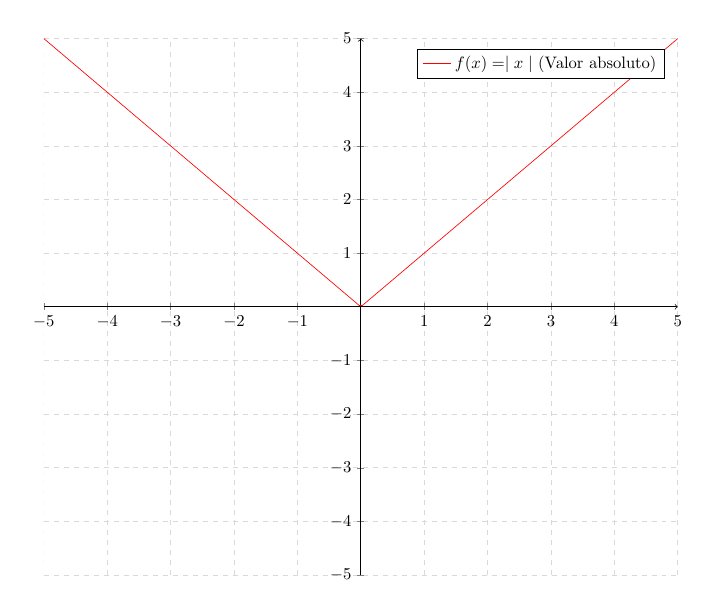
\begin{tikzpicture}[scale=0.6]
            \begin{axis}[
                    axis lines=middle,
                    axis line style={->},
                    %x label style={at={(axis description cs:0.5,-0.06)},anchor=north},
                    %y label style={at={(axis description cs:-0.06,.5)},rotate=90,anchor=south},
                    %xlabel={Nº de bombillas},ylabel={Vida en horas},
                    grid,
                    width=15cm,
                    xmax=5,ymax=5,xmin=-5,ymin=-5,
                    %axis lines=middle
                ]
                \addplot [mark=, samples = 200, red] {abs(x)};
                \addlegendentry{$f(x)=\mid x \mid$ (Valor absoluto)}
            \end{axis}
        \end{tikzpicture}
    \end{multicols}

    \begin{multicols}{2}
        

        % \columnbreak
        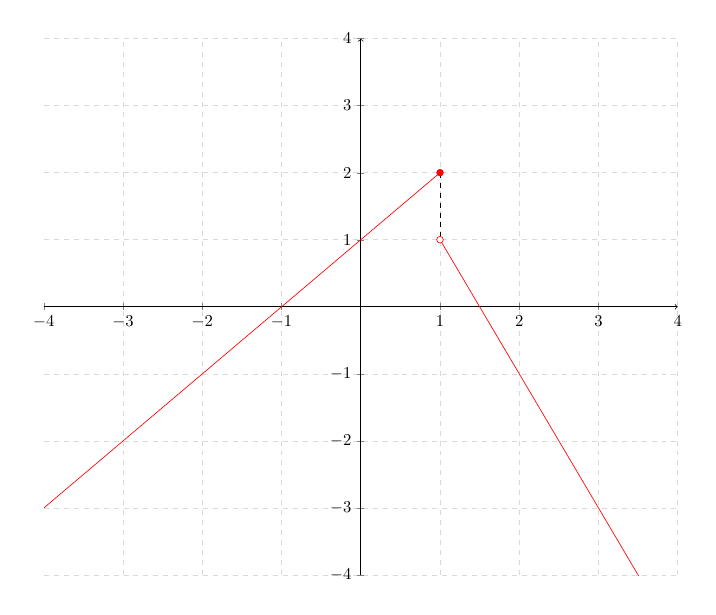
\begin{tikzpicture}[scale=0.6]
            \begin{axis}[
                    %title={$f(x)=x^2-10$},
                    axis lines=middle,
                    axis line style={->},
                    legend style={inner ysep=7pt},
                    %x label style={at={(axis description cs:0.5,-0.06)},anchor=north},
                    %y label style={at={(axis description cs:-0.06,.5)},rotate=90,anchor=south},
                    %xlabel={Nº de bombillas},ylabel={Vida en horas},
                    no markers,
                    grid,
                    width=15cm,
                    xmax=4,ymax=4,xmin=-4,ymin=-4,
                    %axis lines=middle
                    restrict y to domain=-20:20
                ]
                %\addplot [color=green, mark=] {x};
                \addplot [mark= thick,  domain = -10:1, samples=50, red] {x+1};
                \addplot [mark= thick,  domain = 1:10, samples=50, red] {-2*x+3};
                %\addlegendentry{$f(x)=\frac{1}{x}$}

                \draw[dashed] (axis cs:1,2) -- (axis cs:1,1);

                \addplot[holdot] coordinates{(1,1)};
                \addplot[soldot] coordinates{(1,2)};
            \end{axis}
        \end{tikzpicture}

        \begin{tikzpicture}[scale=0.6]
            \begin{axis}[
                    %title={$f(x)=x^2-10$},
                    axis lines=middle,
                    axis line style={->},
                    legend style={inner ysep=7pt},
                    %x label style={at={(axis description cs:0.5,-0.06)},anchor=north},
                    %y label style={at={(axis description cs:-0.06,.5)},rotate=90,anchor=south},
                    %xlabel={Nº de bombillas},ylabel={Vida en horas},
                    no markers,
                    grid,
                    width=15cm,
                    xmax=20,ymax=20,xmin=-20,ymin=-20,
                    %axis lines=middle
                    % restrict y to domain=-20:20
                ]
                \addplot[domain=-15:-5,red] {x+10};
                \addplot[domain=0:4,red] {x*x};
                \addplot[domain=4:6,red] {x};
                \addplot[domain=6:10,red] {-5};
                \draw[dashed] (axis cs:4,16) -- (axis cs:4,4);
                \draw[dashed] (axis cs:6,6) -- (axis cs:6,-5);
                \addplot[holdot] coordinates{(-15,-5)(0,0)(4,4)(6,-5)};
                \addplot[soldot] coordinates{(-5, 5)(4,16)(6,6)(10,-5)};
            \end{axis}
        \end{tikzpicture}
    \end{multicols}
\end{questions}

\end{document}